\documentclass[final,12pt]{article}
\usepackage[utf8]{inputenc}
\usepackage[margin=24mm]{geometry}
\usepackage{polyglossia,titling,graphicx,dingbat}
\usepackage[numbers]{natbib}
\usepackage{xspace}
\usepackage{url}
\usepackage[colorlinks,urlcolor=blue,citecolor=black,linkcolor=black]{hyperref}

\setdefaultlanguage{spanish}

\frenchspacing
\hyphenation{unicode}
%FIXME: todas las figuras se citan con F mayuscula
\date{\today}
% el titulo debe ir orientado a que sera en la region de samalayuca
\title{[TÍTULO DEL PROYECTO DE INVESTIGACIÓN]}
\author{Guillermo Joaquín Álvarez Ordóñez} 

\begin{document}
\thispagestyle{empty}
\begin{center} \vfill
{\Large UNIVERSIDAD AUTÓNOMA DE CIUDAD JUÁREZ}\\
\vspace{6mm}
{\large Instituto de Ingeniería y Tecnología\\
\vspace{6mm}
Departamento de Ingeniería Eléctrica y Computación
\vspace{20mm}


\includegraphics [scale=0.7]{imagenes/escudo-uacj} 
\vspace{10mm}


% Clave: IEC982300B % replace with course code

% Materia: Seminario de Titulación I % replace with course title

% Semestre: Otoño 2017 % replace with term and year of the exam

% Matrícula: 123456 \theauthor \vfill

\thetitle\\
\vspace{15mm}


Protocolo de investigación presentado por:\\
\vspace{6mm}
\theauthor\hspace{10mm} [Matrícula]\\
\vspace{10mm}
Requisito para la obtención del título de\\
\vspace{6mm}
INGENIERO EN SISTEMAS COMPUTACIONALES\\
\vspace{10mm}

Asesor:\\
{[Nombre del asesor]}\\
} \vfill
	Ciudad Juárez, Chihuahua \hspace{70mm}\today

\end{center} 

\clearpage

% \tableofcontents
% \clearpage
% \listoffigures
% \clearpage
% \listoftables
% \clearpage

% \begin{abstract} 
    \noindent
    En la actualidad existen asistentes de voz que son capaces de reconocer comandos o instrucciones a partir de la voz de las personas. Dichos asistentes son usados principalmente para tareas sencillas como búsquedas en Internet o agendas y aún son ineficientes a la hora de reconocer y procesar el contexto en una conversación. En este proyecto se propone implementar un asistente de voz con la capacidad de interpretar el lenguaje natural y seguir una conversación sin salirse de contexto, utilizando \textit{answer sets programming} (ASP). En este documento se muestra la descripción de los asistentes de voz más relevantes actualmente, se da una justificación del proyecto, la metodología, los objetivos generales y el coronograma de actividades a seguir para implementar un prototipo de asistente de voz.
\end{abstract}
     
\section*{Introducción}

"La agricultura es la base de la economía en muchos países, esta provee a la humanidad de algunas de sus necesidades más básicas: comida y fibra" \cite{appsremotesensing}. La demanda de comida y productos derivados de la agricultura está proyectada a incrementar en un 70\% para el año 2050 \cite{wik_pingali_brocai_2008}. La agricultura de precisión (PA por sus siglas en inglés) es clave para poder alcanzar la agricultura sustentable. La PA se puede definir como una estrategia de manejo que implementa la recopilación de información, comunicación entre sistemas y técnicas de análisis de datos para apoyar la toma de decisiones, por ejemplo: aplicación de fertilizantes, control de plagas, control de riego, identificación de enfermedades, entre otros \cite{appsremotesensing}.

Actualmente existen varios sistemas en el mercado para el control y monitoreo de invernaderos o cuartos de producción. Los sistemas básicos ofrecen monitoreo de temperatura, humedad, CO2, e intensidad de la luz, con un costo de \$2,159.90 USD y \$2,351.00 USD respectivamente \cite{intelliclimate_kit_2021}, \cite{smartbee_kit_2021}. Ambos sistemas se pueden conectar a internet para realizar un monitoreo remoto, alertar cuando las condiciones salgan de los límites definidos e iniciar las acciones correctivas correspondientes, sin embargo, \cite{intelliclimate_kit_2021} necesitará una interfaz y una subscripción extra, añadiendo \$279.00 USD al costo. 

Existen otras alternativas, sin embargo, estas ofrecen un servicio similar excepto a escala industrial \cite{ceres_greenhouse_solutions_2021}, \cite{autogrow_climate_control_2021}, \cite{climate_control_2021}. Debido a su mercado objetivo, estos sistemas industriales solo ofrecen cotizaciones a clientes potenciales.

En junio de 2020 se realizó una encuesta (\ref{encuesta}) en la que participó un grupo de agricultores de escala pequeña y mediana, ubicados en Samalayuca, Chihuahua. El 87.6\% de los sondeados no cuentan con un sistema de riego automatizado. Al 76.1\% les gustaría un sistema de ventilación automatizado. Los primeros tres parámetros que se consideraron más importantes de monitorear fueron los siguientes: temperatura del ambiente, humedad del ambiente y la humedad del suelo. Al 84.1\% les gustaría controlar y monitorear sus cultivos desde su teléfono o computadora, sin embargo, casi el 90\% de los encuestados no están dispuestos a adquirir un sistema a costo del mercado.

%FIXME: agregar un parrafo intermedio

La comunicación inalámbrica entre sistemas ha cambiado los estándares de comunicación al día de hoy y la agricultura no se ha quedado atrás. "Para incrementar la eficiencia, productividad y reducir la intervención humana, tiempo y costo existe una necesidad de prestar atención a una nueva tecnología llamada Internet de las Cosas (\textit{IoT} por sus siglas en inglés)" \cite{agriculture_automation_review}. El IoT es la red de dispositivos que adquieren y actúan sobre información sin la necesidad de que un humano intervenga \cite{agriculture_automation_review}. 

Los principales componentes de un sistema basado en \textit{IoT} se pueden dividir en 4 capas: dispositivos, red, servicios y aplicación. El \textit{hardware} a implementar es de suma importancia debido a que impacta directamente el costo de la implementación y restringe las tecnologías disponibles. Entre los dispositivos más utilizados están los diferentes Arduinos, Raspberry Pis y el microcontrolador ESP. Los datos obtenidos a través de estos dispositivos son (en su mayoría) enviados a una ubicación central a través de una red alámbrica o inalámbrica. Los principales protocolos de red implementados en las redes inalámbricas son: Wi-Fi, Bluetooth, Zigbee y LoRaWAN \cite{systematicreviewiot}. 

\section{Planteamiento del problema}

\subsection{Antecedentes}

"La agricultura es la base de la economía en muchos países, esta provee a la humanidad de algunas de sus necesidades más básicas: comida y fibra" \cite{appsremotesensing}. 
La demanda de comida y productos derivados de la agricultura está proyectada a incrementar en un 70\% para el año 2050 \cite{wik_pingali_brocai_2008}. 
La agricultura de precisión (PA por sus siglas en inglés) será clave para poder alcanzar la agricultura sustentable. La PA se puede definir como una 
estrategia de manejo que implementa la recopilación de información, comunicación entre sistemas y técnicas de análisis de datos para apoyar la toma 
de decisiones, por ejemplo: aplicación de fertilizantes, control de plagas, control de riego, identificación de enfermedades, entre otros \cite{appsremotesensing}.

La comunicación inalámbrica entre sistemas ha cambiado los estándares de comunicación a día de hoy y la agricultura no se ha quedado atrás. 
"Para incrementar la eficiencia, productividad y reducir la intervención humana, tiempo y costo existe una necesidad de prestar atención a una
nueva tecnología llamada Internet de las Cosas (\textit{IoT} por sus siglas en inglés)" \cite{agriculture_automation_review}. El IoT es la red de dispositivos 
que adquieren y actúan sobre información sin la necesidad de que un humano intervenga \cite{agriculture_automation_review}. 

Los principales componentes de un sistema basado en \textit{IoT} se pueden dividir en 4 capas: dispositivos, red, servicios y aplicación. 
El \textit{hardware} a implementar es de suma importancia debido a que impacta directamente el costo de la implementación y restringe 
las tecnologías disponibles. Entre los dispositivos más utilizados están los diferentes Arduinos, Raspberry Pis y el microcontrolador ESP. 
Los datos obtenidos a través de estos dispositivos son (en su mayoría) enviados a una ubicación central a través de una red alámbrica o inalámbrica.
Los principales protocolos de red implementados en las redes inalámbricas son: Wi-Fi, Bluetooth, Zigbee y LoRaWAN \cite{systematicreviewiot}. 

En \cite{olive_orchard_monitorization} se implementó una red inalámbrica de sensores de bajo costo para monitorear la temperatura, humedad y concentración de gases 
del ambiente, además de la humedad del suelo en una plantación de olivos. Se utilizó el sensor DHT 11 para monitorear la temperatura y humedad del ambiente, un
higrómetro para medir la humedad del suelo y un MQ-135 para detectar gases nocivos (CO2, amoniaco, benzeno, alcohol y humo del fuego). Cada nodo de esta 
red cuenta con los sensores para realizar las lecturas mencionadas, un microcontrolador y una antena para habilitar la comunicación mediante el protocolo 
LoRaWAN, todo alimentado por celdas fotovoltaicas. Para el monitoreo de las lecturas, se desarrollaron una aplicación móvil y una interfaz web que 
muestran los datos en tiempo real.

Es importante monitorear de forma separada la humedad del ambiente como la humedad del suelo debido a que estas no están correlacionadas. Ambas se relacionan
a enfermedades y plagas, sin embargo, la humedad del ambiente influye en la aparición de enfermedades y la humedad del suelo en la aparición de plagas. También
es muy valioso contar con mediciones de temperatura cerca del cultivo. De esta manera se tienen datos más precisos que los que proveen los sitios/aplicaciones 
meteorológicas \cite{olive_orchard_monitorization}.

En la Universidad de Magdalena, Colombia se creó un sistema de bajo costo para monitoreo y control remoto de un invernadero utilizando lógica difusa \cite{low_cost_fuzzy_logic_greenhouse}. La utilización de lógica difusa en sistemas de control permite traducir variables a sets previamente definidos que contienen la 
terminología difusa como muy frío, frío, caliente, muy caliente, etcétera. Gracias a esta traducción se pueden tomar acciones más precisas para realizar el control \cite{agriculture_automation_review}. El algoritmo difuso se implementó en un Arduino Mega para tomar acciones de control sobre la temperatura y humedad del ambiente, humedad del suelo e iluminación. Además, se diseño un sitio web para realizar el monitoreo y poder tomar acciones que sobre escriban a las decisiones tomadas por el sistema. Se probó la efectividad de la lógica difusa para controlar sistemas no lineales, además de optimizar el uso de recursos en un invernadero \cite{low_cost_fuzzy_logic_greenhouse}.

% buscar antecedentes de sistemas existentes que sean costosos para que la metrica sea el bajo costo del objetivo

\subsection{Definición del problema}

% si el objetivo es disminuir el costo aqui puedo argumentar que el costo de sistemas es muy alto
% restringir las afirmaciones que se hagan a donde se implementara el invernadero. Usar encuestas del proyecto de PITI para demostrar que las personas de

%% Sistema de control y monitoreo de un invernadero basado en el Internet de las cosas y logica difusa



% problema de investigacion, no del contexto. No esta ligado directamente al objetivo
La agricultura en Samalayuca, Chihuahua, se basa, en su mayoría, en métodos tradicionales o populares. Esto dificulta que los agricultores
locales puedan competir contra extranjeros que producen en ambientes controlados y automatizados, ya que no pueden igualar ni la calidad 
del producto ni la cantidad producida. Lamentablemente, esto afecta aún más a pequeños y medianos productores ya que los sistemas de control 
y monitoreo son muy costosos.

% La agricultura en Samalayuca, Chihuahua, se basa, en su mayoría, en métodos tradicionales o populares. Esto impacta de forma negativa a los 
% productores de pequeña o mediana escala ya que no cuentan con las herramientas para tomar decisiones basadas en información. Al no contar con 
% información, el replicar resultados en temporada tras temporada es complicado.

% Una toma de decisiones informada ayudará a los agricultores a utilizar de una forma más eficiente sus recursos, disminuyendo el costo de producción. 
% Además, al llevar sistematizar la producción se tendrán resultados replicables temporada tras temporada.

\subsection{Objetivo}
% lo que diga mi objetivo tiene que resolver mi problema al 100% - Como medir el resultado? 
% Utilizando tecnicas de logica difusa
Implementar un sistema de bajo costo para controlar y monitorear el clima de un invernadero utilizando técnicas de lógica difusa.
\section{Objetivo general}
Desarrollar un sistema de bajo costo para controlar y monitorear el clima de un invernadero, ubicado en el rancho El Sufrido, Samalayuca, utilizando técnicas de lógica difusa.

\subsection{Objetivos específicos}
\begin{itemize}
	\item Diseñar, desarrollar e implementar una red inalámbrica de sensores de bajo costo para monitorear el clima de un invernadero.
	\item Desarrollar un API para filtar y enviar los datos obtenidos de los sensores a la nube.
	\item Desarrollar un API para recibir y guardar los datos enviados por la computadora central.
	\item Automatizar el control del invernadero utilizando técnicas de lógica difusa.
	\item Diseñar una interfaz gráfica para monitorear y controlar el clima del mismo de forma remota.
\end{itemize}
\section{Justificación}

% ayudaria, contribuiria utilizar este tipo de verbos copreterito

% la primera oración sigue en pareciendo problema.
Debido a la creciente demanda de alimentos \cite{wik_pingali_brocai_2008}, es imperativo que los agricultores de Samalayuca, Chihuahua, cuenten con herramientas de bajo costo que les permitan tomar decisiones basadas en información. El monitoreo constante de los parámetros que tienen mayor influencia sobre el cultivo les ayudará a identificar situaciones que puedan fomentar la aparición de enfermedades. Asimismo, la automatización de tareas que demandan constancia y precisión, como lo son el riego y el control del clima, contribuirá a la estabilización de estos parámetros, disminuyendo el estrés provocado en las plantas. Esto permitirá que los agricultores locales puedan competir contra extranjeros que producen en ambientes controlados y automatizados. 

Esta solución tendrá un impacto económico ya que podrá ser fácilmente replicada en otros invernaderos donde exista un clima similar. Para regiones con climas distintos, se podrán adaptar las reglas de control para las necesidades particulares de la región. Asimismo, este sistema continuará siendo atractivo para quienes busquen una solución de bajo costo. En la Figura \ref{fig:costo_estimado} se puede observar el costo estimado que tendrán los componentes del proyecto.


\begin{figure}[!ht]
    \centering
    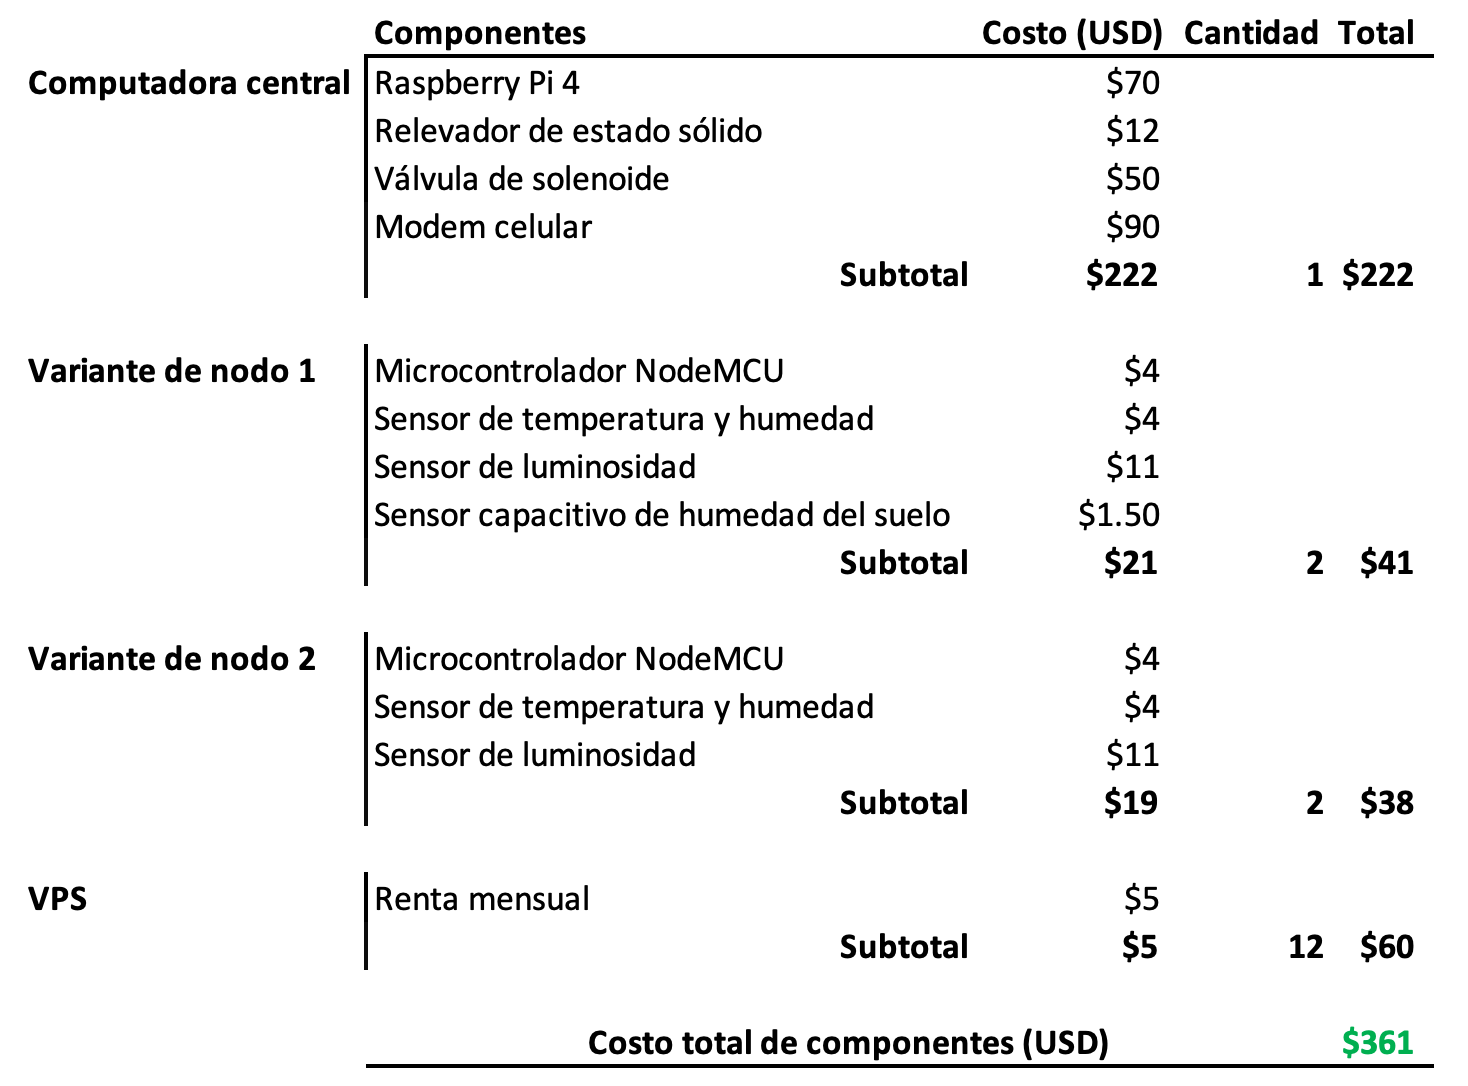
\includegraphics[width=1\linewidth]{imagenes/costo_estimado_proyecto.png}
    \caption{Costo estimado del proyecto }
    \label{fig:costo_estimado}
\end{figure}




\section{Propuesta de solución}

Se desarrollará un sistema de bajo costo para monitorear y controlar el clima de un invernadero a través de técnicas de lógica difusa.

El monitoreo se basará en una red inalámbrica de sensores. Esta red estará compuesta de una computadora central y nodos que realizarán las lecturas de los distintos sensores y enviarán los datos a través de Wi-Fi a la computadora central. Esta computadora estará encargada de actuar como punto de acceso para todos los nodos, siendo la única con conexión a internet. 

Esta será un \textit{raspberry pi} 4, estará encargada de recibir los datos, procesarlos, filtrarlos y enviarlos a un servidor en la nube. En esta computadora también se realizará el control difuso del riego y del clima, tomando decisiones a partir de las lecturas de sensores y las reglas heurísticas previamente definidas. Este control podrá ser sobre escrito a través de la interfaz de usuario, conservando así total control sobre el sistema.

Existirán 2 variantes de nodos. Ambas variantes contarán con un microcontrolador Node MCU-ESP8266, el cual estará encargado de sensar un sensor de temperatura y humedad (DHT11), un sensor de intensidad de luz (Adafruit 4162 VEML7700) y, dependiendo de la variante, un sensor capacitivo de humedad del suelo. Los nodos estarán dispersos uniformemente dentro del invernadero, los que cuenten con sensor de humedad del suelo estarán a nivel del suelo y los que no, estarán a una altura en la que el cultivo no cubra el sensor de iluminancia.

En el servidor alojado en la nube se encontrará una interfaz para programas de aplicación (API por sus siglas en inglés) REST codificada en NodeJS. Esta se encargará de recibir los datos enviados por la computadora central del invernadero y guardarlos en una instancia de MongoDB. Estos datos serán los que el usuario podrá monitorear en la interfaz, así como realizar el control remoto a través de un túnel inverso SSH.

\section{Marco teórico}
%\caption[Texto en lista de figuras sin cita]{Texto en título de imagen con cita.}

[Presentar la teoría que va a fundamentar el proyecto con base en le planteamiento del problema que se ha realizado, los conceptos y conocimientos necesarios para desarrollar el proyecto. Se puede dividir en sub-secciones por cada concepto que se necesite, pero no olvides introducir antes con un párrafo.]
\section{Alcances y limitaciones}

\subsection*{Alcances}
\begin{itemize}
    \item El sistema solo monitoreará 4 variables dentro de un invernadero: temperatura ambiental, humedad del suelo, humedad ambiental e intensidad de la luz.
    \item Se controlará el riego del mismo utilizando una válvula de solenoide y el clima a través de abanicos y aspersores de niebla utilizando técnicas de lógica difusa. 
    \item La interfaz web no será multi-usuario.
    \item Solamente va a operar en el invernadero del rancho el sufrido
    \item Estos datos podrán ser monitoreados y controlados en tiempo real solamente a través de una interfaz web.
    \item En la interfaz, se podrán consultar datos históricos sobre las mediciones.
    \item Juntar los ultimos 3 puntos
    \item Narrarlo desde la perspectiva de los datos historicos: los datos historicos sobre las maediciones se podran consultar a traves de la interfaz web
\end{itemize}

\subsection*{Limitaciones}
\begin{itemize}
    \item El funcionamiento del sistema estará sujeto a disponibilidad de energía eléctrica.
    \item El envío de datos al servidor en la nube estará sujeto a disponibilidad de internet.
    \item No se realizará ningún tipo de control sobre la intensidad de la luz, principalmente por limitantes económicas.
    \item El control y monitoreo hecho a través de la interfaz web estará sujeto a disponibilidad de internet por parte del usuario y del servidor.
\end{itemize}

\section{Metodología}

Modelo en cascada

Análisis 
    - Los parámetros que les importan a los agricultores los puedo sacar de unas encuestas
Diseño
    - Agregar imágenes de los sensores y agregar diagramas de la arquitectura que tendrá el sistema
Implementación
    - El microcontrolador se programará en Arduino, los datos se enviarán a través de HTTP
    - En el rapberry puedo usar python (dependerá de las librerías de lógica difusa)
    - En el servidor en la nube se utilizará un api en nodejs y se guardarán los datos en Mongo
    - Para el front se va a utilizar Vuejs, el cual consultará los datos al API en la nube (se va a usar NGINX como servidor web)

    - 



\section{Programa de Actividades}
Las actividades, con sus tiempos respectivos, para llevar a cabo este proyecto se encuentran detalladas en el Cuadro 1.

\begin{table}[ht]
	\label{tbl:actividades}
    \centering
	\resizebox*{!}{17 cm}{
		\begin{tabular}{|p{8cm}|c|c|c|c|c|c|c|c|c|c|}
			\hline 
			ACTIVIDAD&\rotatebox{90}{Febrero 2021}
			&\rotatebox{90}{Marzo}
			&\rotatebox{90}{Abril} 
			&\rotatebox{90}{Mayo} 
			&\rotatebox{90}{Junio} 
			&\rotatebox{90}{Julio} 
			&\rotatebox{90}{Agosto} 
			&\rotatebox{90}{Septiembre} 
			&\rotatebox{90}{Octubre} 
			&\rotatebox{90}{Noviembre 2021}\\
			\hline
			Revisión de la Literatura&\checkmark &\checkmark  &\checkmark  &  &  &  &  &  & &  \\  
			\hline
			Protocolo&\checkmark &\checkmark  &\checkmark  &  &  &  &  &  & &  \\  
			\hline 
			Selección de software existente&\checkmark &\checkmark  &  &  &  &  &  &  & &  \\  
			\hline 
			Selección de hardware existente&\checkmark &\checkmark  &  &  &  &  &  &  & &  \\  
			\hline 
			Documentación de propuesta&  &  & \checkmark & \checkmark &\checkmark  &\checkmark  &\checkmark  &\checkmark  &\checkmark  &\checkmark  \\ 
			\hline 
			Diseño de la red inalámbrica&  &  &  & \checkmark &  &  &  &  &  &  \\ 
			\hline 
			Desarrollo de la red inalámbrica&  &  &  & \checkmark &  &  &  &  &  &  \\ 
			\hline 
			Pruebas de la red inalámbrica&  &  &  & \checkmark &  &  &  &  &  &  \\ 
			\hline 
			Implementación de la red inalámbrica&  &  &  & \checkmark &  &  &  &  &  &  \\ 
			\hline 
			Desarrollo del API REST de la computadora central&  &  &  &  & \checkmark  &  &  &  &  &  \\ 
			\hline 
			Pruebas del API REST de la computadora central&  &  &  &  & \checkmark  &  &  &  &  &  \\ 
			\hline 
			Implementación del API REST de la computadora central&  &  &  &  & \checkmark  &  &  &  &  &  \\ 
			\hline 
			Desarrollo del API REST del servidor en la nube&  &  &  &  & \checkmark &  &  &  &  &  \\ 
			\hline 
			Pruebas del API REST del servidor en la nube&  &  &  &  & \checkmark &  &  &  &  &  \\ 
			\hline 
			Implementación del API REST del servidor en la nube&  &  &  &  & \checkmark &  &  &  &  &  \\ 
			\hline 
			Investigación y aprendizaje sobre Lógica difusa&  &  &  & \checkmark &\checkmark  &\checkmark  &  &  &  & \\ 
			\hline 
			Formulación de semántica para razonamiento difuso&  &  &  &  &  &\checkmark  &  &  &  &  \\ 
			\hline 
			Automatización del control mediante técnicas de lógica difusa&  &  &  &  &  &  &  \checkmark & \checkmark &  &  \\ 
			\hline  
			Diseño de aplicación web para monitorear y controlar el invernadero de forma remota&  &  &  &  &  &  &  &  & \checkmark  &  \\ 
			\hline  
			Desarrollo de aplicación web para monitorear y controlar el invernadero de forma remota&  &  &  &  &  &  &  &  & \checkmark &  \\ 
			\hline  
			Presentación y defensa de trabajo&  &  &  &  &  &  &  &  &  & \checkmark  \\ 
			\hline
		\end{tabular}
	}
	\caption{Actividades a diez meses}
\end{table}

\bibliography{referencias}
\bibliographystyle{ieeetr}

\clearpage
\appendix
\section{Apéndice}
\subsection{Encuesta realizada a agricultores de Samalayuca, Chihuahua.}

\begin{figure}[!h]
	\centering
	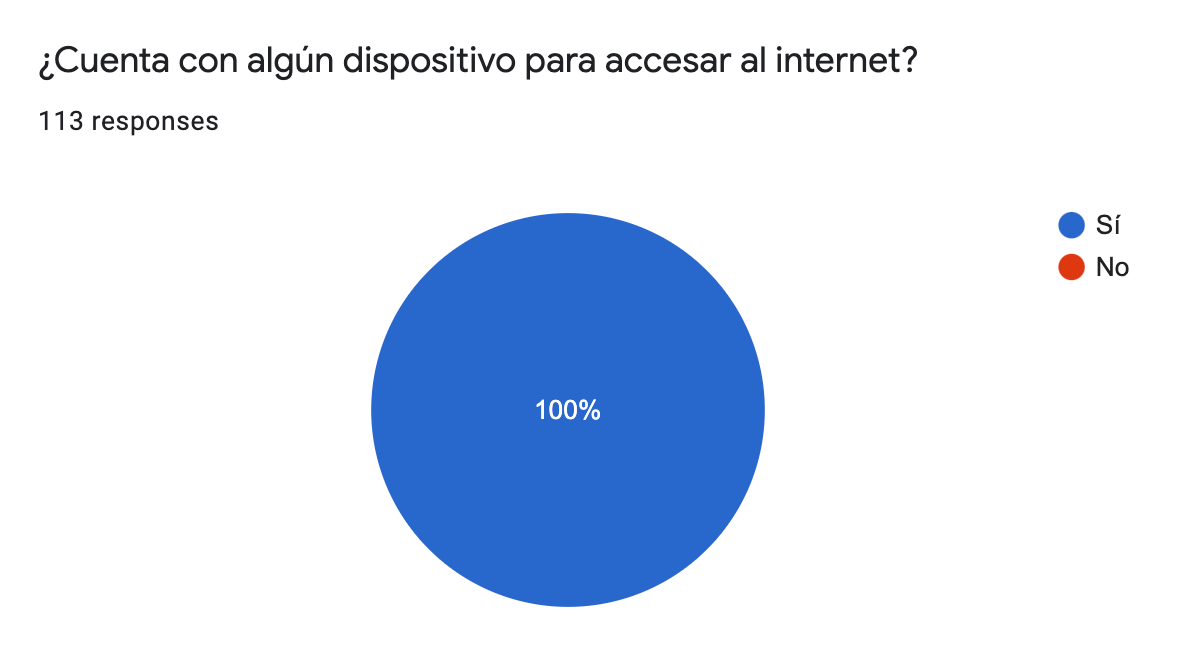
\includegraphics[width=.95\linewidth]{imagenes/encuesta/pregunta_1.png}
	\caption{Resultados de la pregunta ¿Cuenta con algún dispositivo para accesar a internet?}
	\label{fig:pregunta_1}
\end{figure}

\begin{figure}[!h]
	\centering
	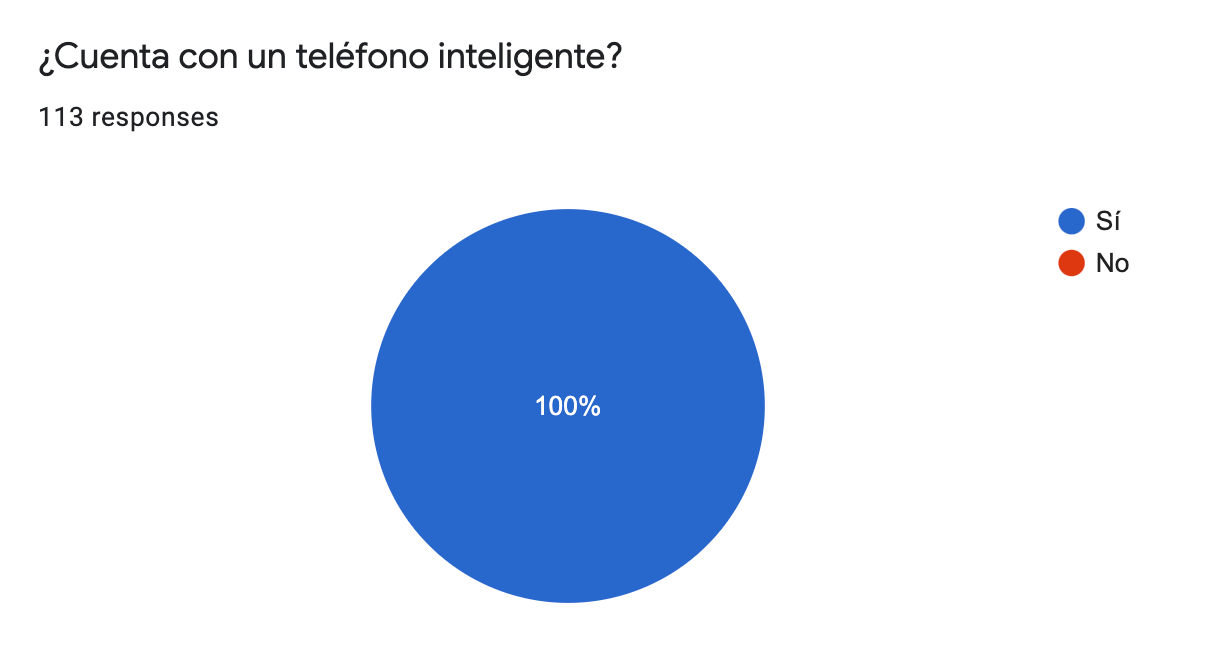
\includegraphics[width=.95\linewidth]{imagenes/encuesta/pregunta_2.png}
	\caption{Resultados de la pregunta ¿Cuenta con un teléfono inteligente?}
	\label{fig:pregunta_2}
\end{figure}

\begin{figure}[!h]
	\centering
	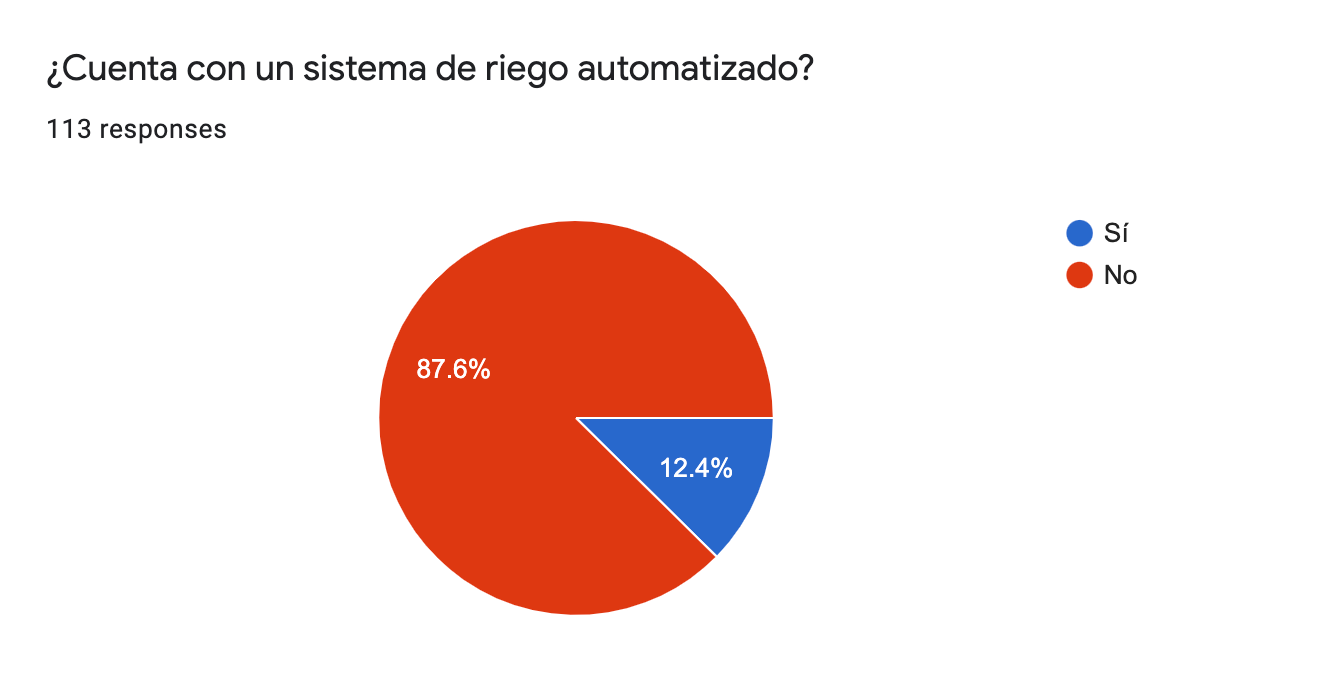
\includegraphics[width=1\linewidth]{imagenes/encuesta/pregunta_3.png}
	\caption{Resultados de la pregunta ¿Cuenta con un sistema de riego automatizado?}
	\label{fig:pregunta_3}
\end{figure}

\begin{figure}[!h]
	\centering
	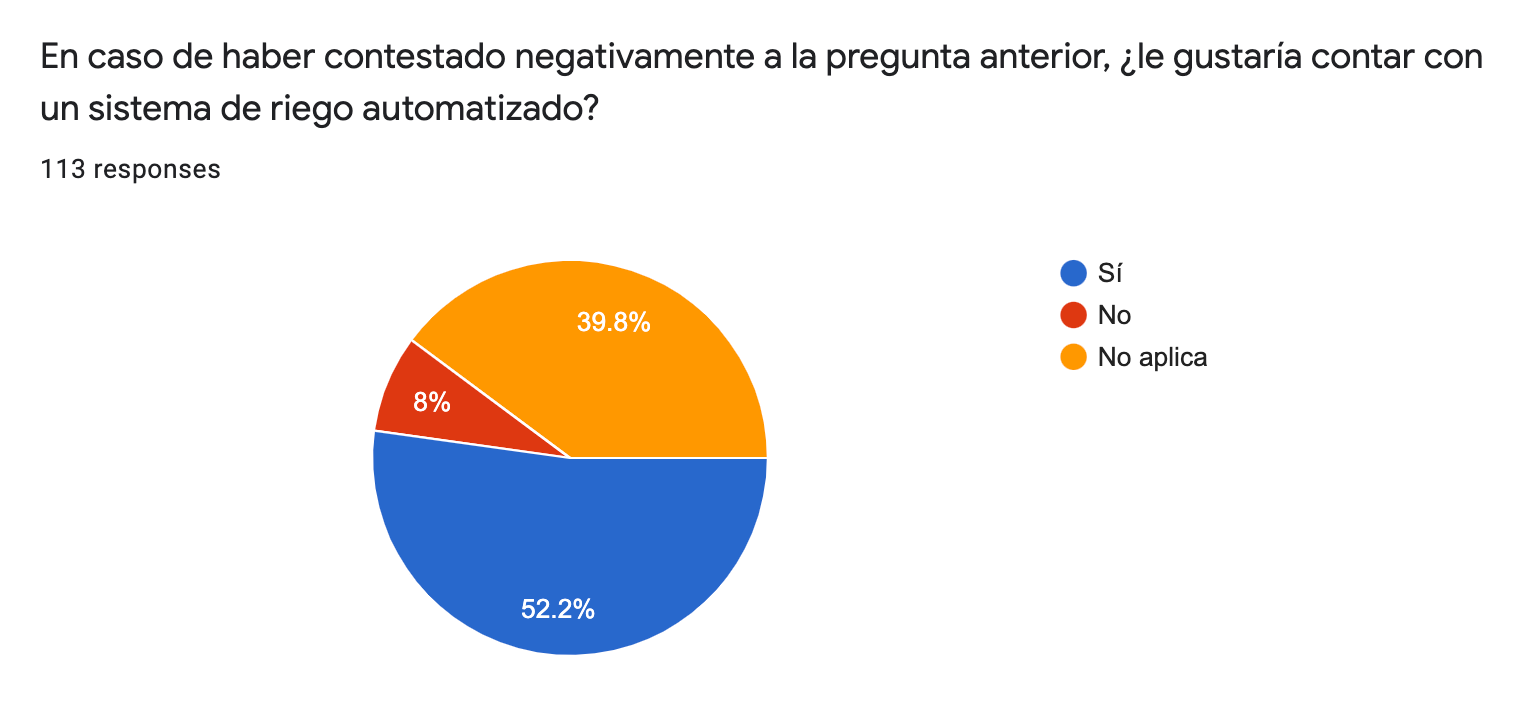
\includegraphics[width=1\linewidth]{imagenes/encuesta/pregunta_4.png}
	\caption{Resultados de la pregunta ¿Le gustaría contar con un sistema de riego automatizado?}
	\label{fig:pregunta_4}
\end{figure}

\begin{figure}[!h]
	\centering
	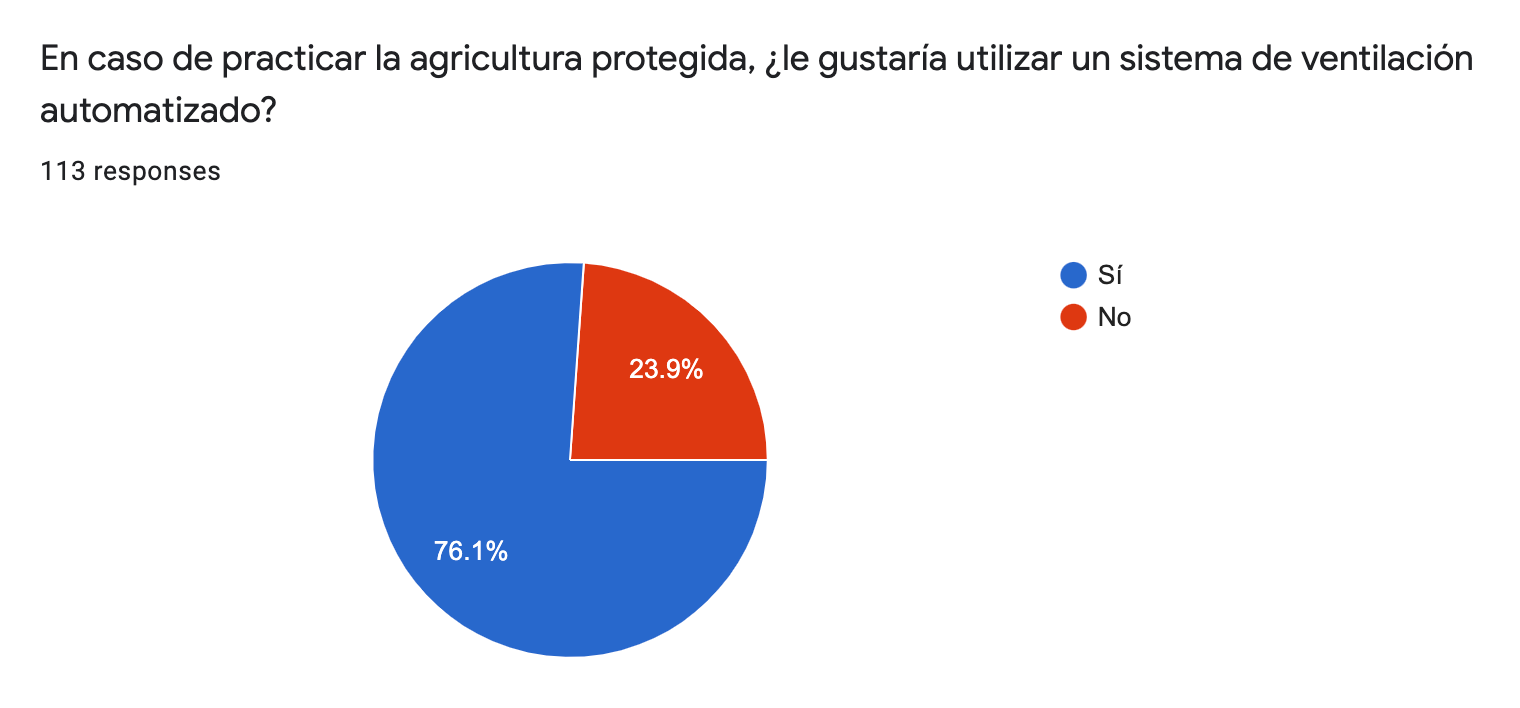
\includegraphics[width=1\linewidth]{imagenes/encuesta/pregunta_5.png}
	\caption{Resultados de la pregunta ¿Le gustaría contar con un sistema de ventilación automatizado?}
	\label{fig:pregunta_5}
\end{figure}

\begin{figure}[!h]
	\centering
	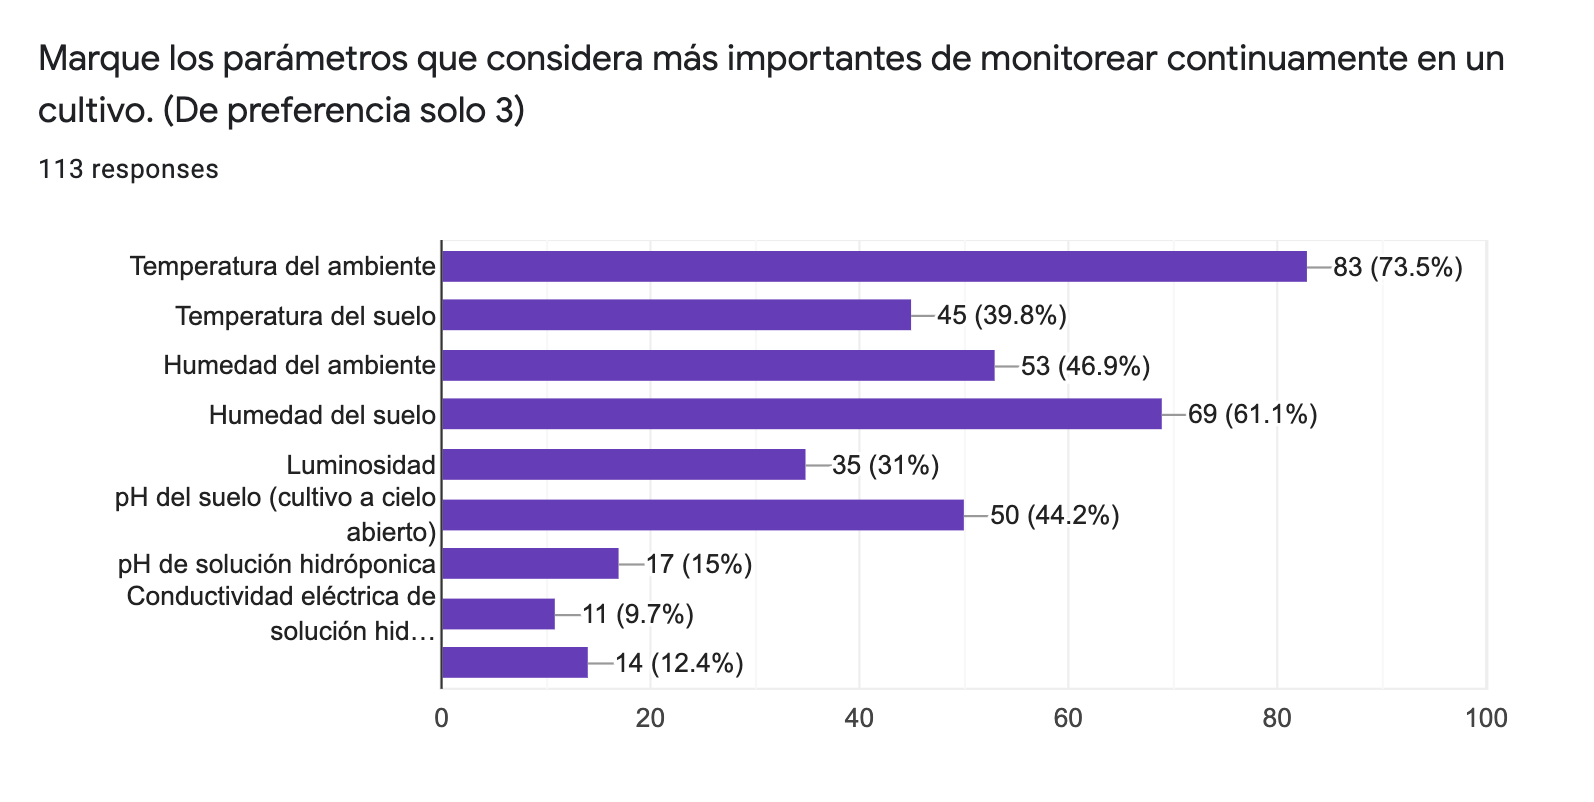
\includegraphics[width=1\linewidth]{imagenes/encuesta/pregunta_6.png}
	\caption{Parámetros considerados como los más importantes de monitorear.}
	\label{fig:pregunta_6}
\end{figure}

\begin{figure}[!h]
	\centering
	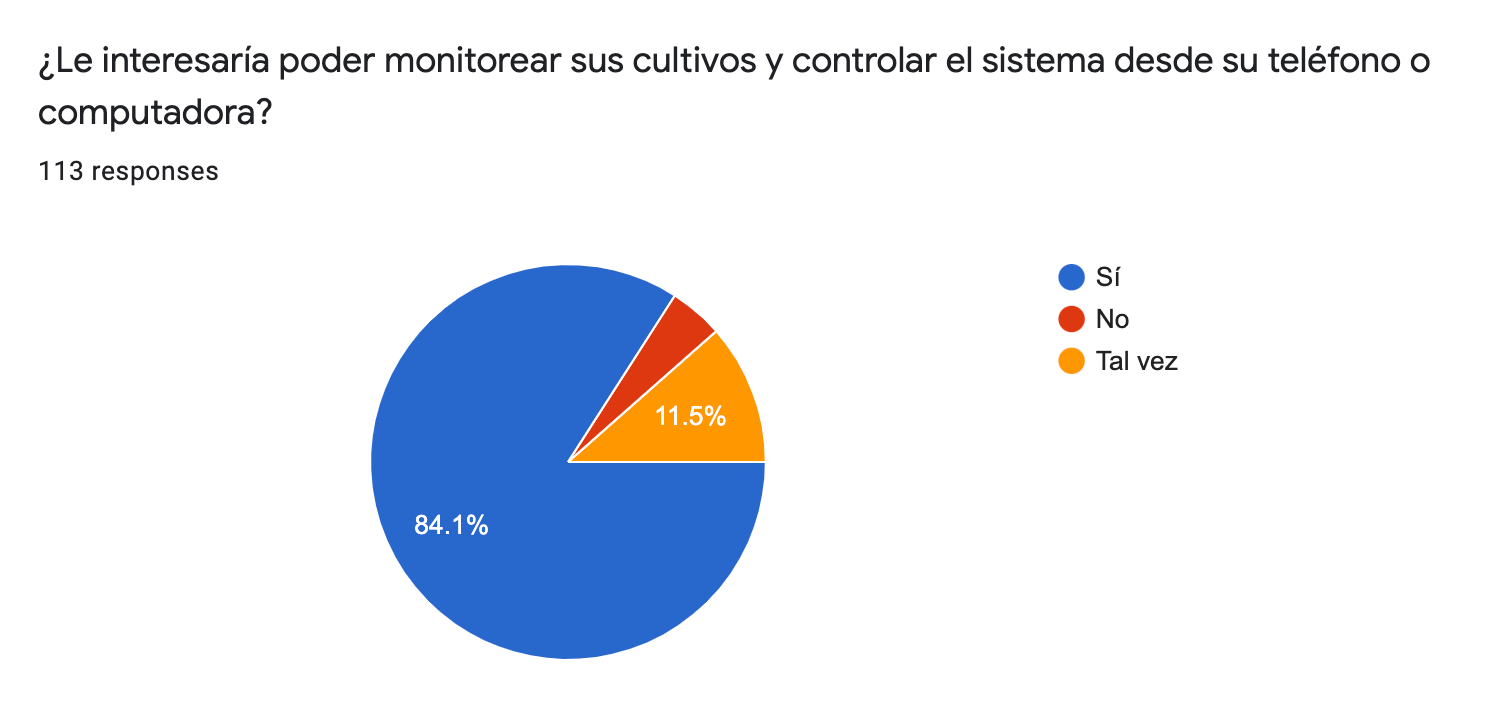
\includegraphics[width=1\linewidth]{imagenes/encuesta/pregunta_7.png}
	\caption{Resultados de la pregunta ¿Le interesaría poder monitorear sus cultivos y controlar el sistema desde su teléfono o computadora?}
	\label{fig:pregunta_7}
\end{figure}

\begin{figure}[!h]
	\centering
	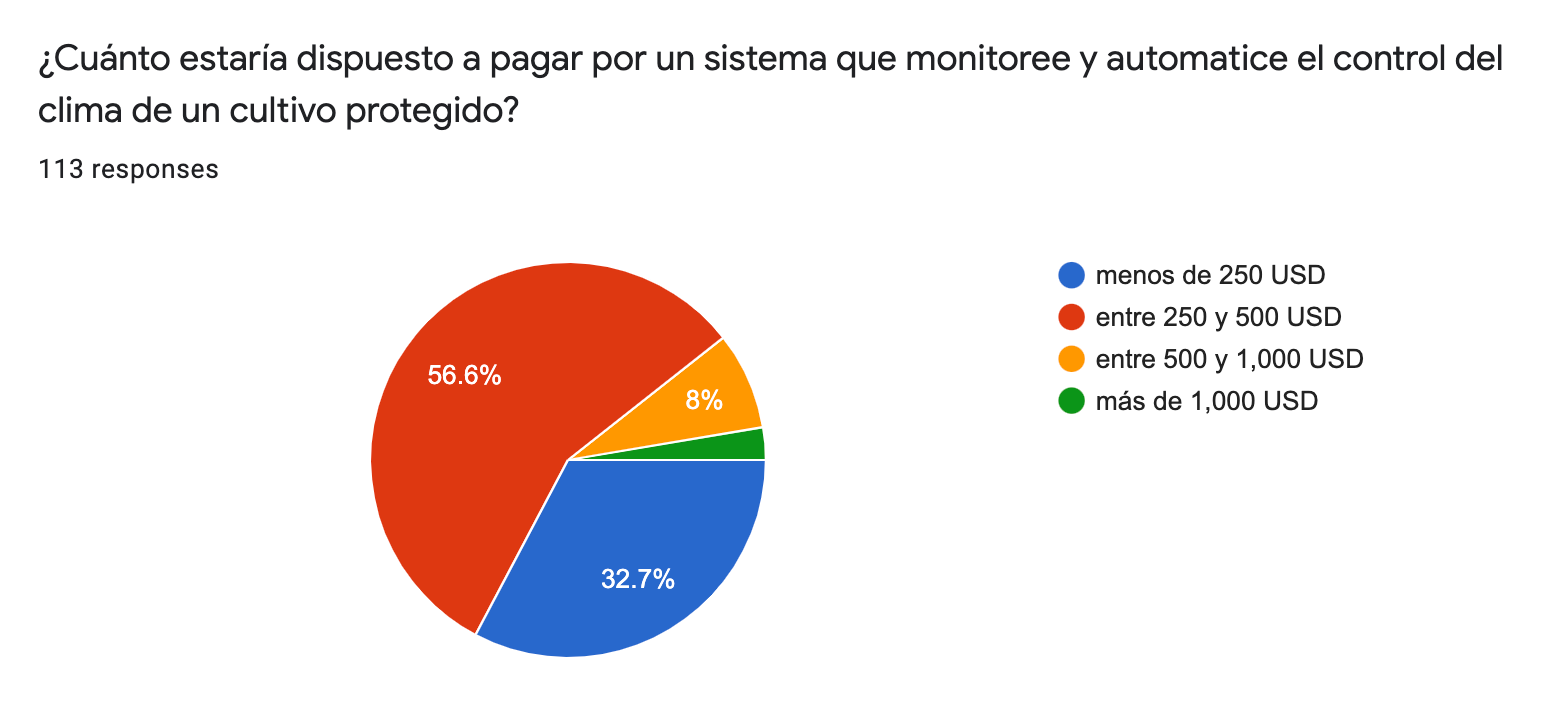
\includegraphics[width=1\linewidth]{imagenes/encuesta/pregunta_8.png}
	\caption{Resultados de la pregunta ¿Cuánto estaría dispuesto a pagar por un sistema que monitoree y automatice el clima de un cultivo protegido?}
	\label{fig:pregunta_8}
\end{figure}



\end{document}